
\section{System Overview}

After pre-processing steps, including raw text collection and tokenization of paragraphs, sentences, and words, we build off of four content selection methods. One is our baseline, Lead-$k$, which simply takes the first $k$ sentences in a document. Two use a extractive approach and build off of a shared TF-IDF class: Integer Linear Programming (ILP) \& LexRank. The fourth content selection model uses an abstractive approach, using gap sentence generation on a large language model. It has a direct connection with the ROUGE score as it uses it to figure out the importance of sentences during training.

Lead-$k$, ILP, and LexRank all use clustering and coreference resolution as information ordering and content realization methods respectively. The large language model uses a sequence to sequence model to improve upon information ordering and content realization together.

Figure \ref{SystemArchitecture} provides an illustration of our system architecture.

\begin{figure}[h]
    \centering
    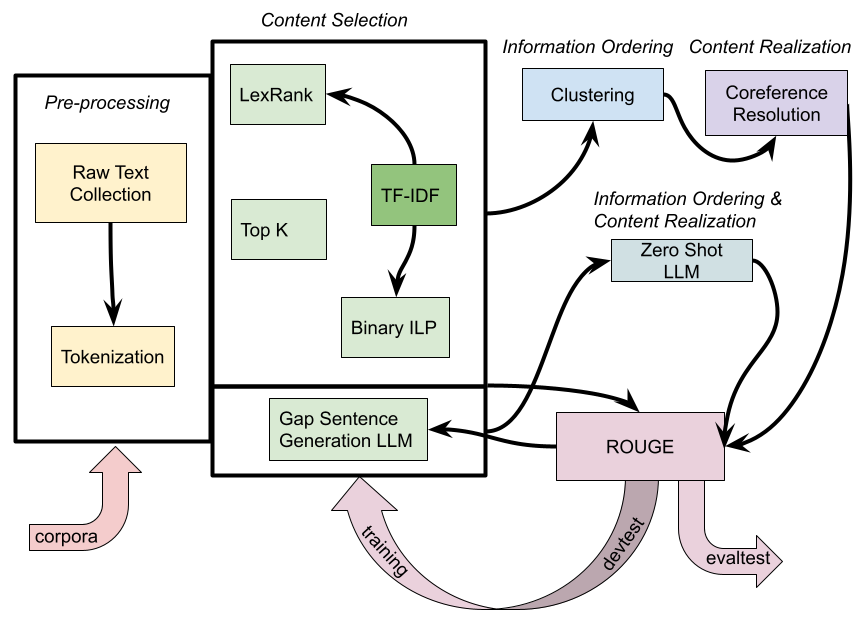
\includegraphics[scale=0.24]{D5_ System Architecture.png}
    \caption{The base system architecture from preprocessing the data to content realization}
    \label{SystemArchitecture}
\end{figure}